El Sistema de Energ�a se encarga de almacenar, distribuir y acondicionar la energ�a el�ctrica para todos los componentes del CanSat. Se debe tener en cuenta que dentro del CanSat existe una cantidad considerable de dispositivos electr�nicos como sensores, indicadores, motores, entre otros, los cuales tienen la finalidad de trabajar en conjunto para cumplir los requerimientos de la misi�n. Estos dispositivos trabajan a diferentes niveles de tensi�n, por lo que se debe asegurar que �ste sea el adecuado para cada uno.\\

\noindent En la figura \ref{fig:DiagramaCansat} se presentan los componentes relacionados con las distribuci�n y acondicionamiento de energ�a en el CanSat. El MOSFET de canal P tiene la finalidad de proteger el circuito el�ctrico de una polarizaci�n inversa (conectar las terminales de la bater�a al rev�s). Como se puede ver en la figura \ref{fig:DiagramaCansat}, el voltaje de entrada al CanSat es de $ 9 [V] $ y, al pasar por toda la circuiter�a respectiva, se producen dos salidas de tensi�n: una a $6 [V]$ y la otra a $3.3 [V]$.

\begin{figure}[H]
\begin{center}
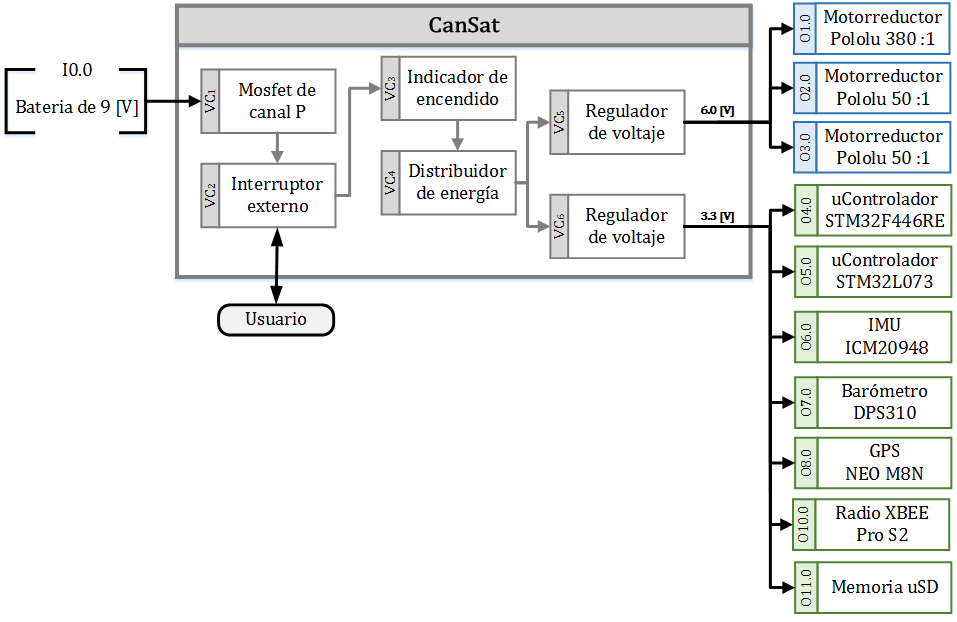
\includegraphics[scale=0.5]{diseniosist/SEn/DiagramaCansat.png}  
\caption{Representaci�n a bloques de los componentes electr�nicos del CanSat y su respectiva tensi�n de alimentaci�n. \label{fig:DiagramaCansat}}
\end{center}
\end{figure}

En la figura \ref{fig:DiagramaRegulacion} se muestra un extracto de la figura \ref{img:EsquematicoPP} presentada en la secci�n \ref{sistSPD} que corresponde al circuito el�ctrico encargado de regular el voltaje de entrada de $9 [V]$ a $3.3 [V]$ y $6 [V]$. En la figura \ref{fig:DiagramaRegulacion} se logra ver el MOSFET de protecci�n $Q1$, el interruptor principal $SW1$, y los reguladores de voltaje $U3$ y $U4$ para $6 [V]$ y $3.3 [V]$, respectivamente.

\begin{figure}[H]
	\begin{center}
		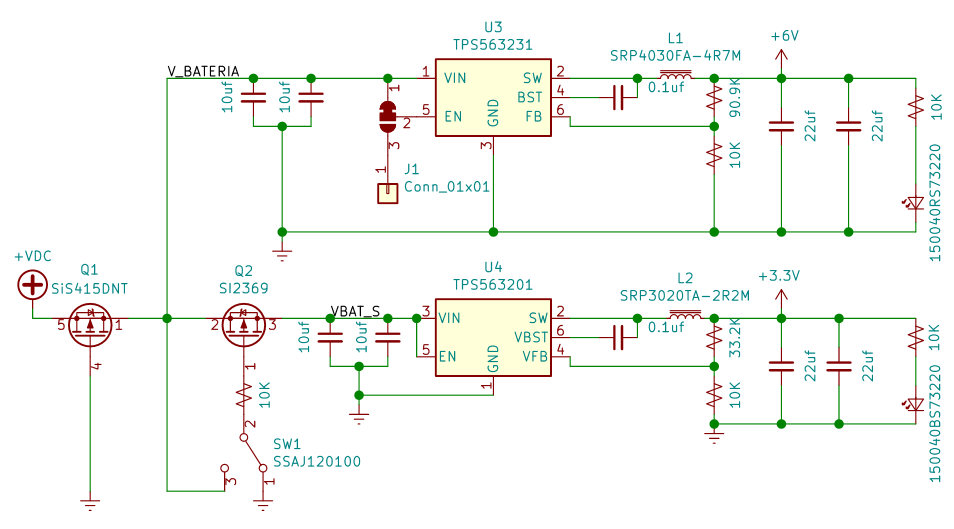
\includegraphics[scale=0.5]{diseniosist/SEn/reguladores.png}  
		\caption{Circuito el�ctrico para regular la tensi�n de $9 [V]$ a $3.3 [V]$ y $6 [V]$. \label{fig:DiagramaRegulacion}}
	\end{center}
\end{figure}

\noindent En la Tabla \ref{tab:ConsumoCansat} se presenta el consumo de energ�a de cada uno de los dispositivos electr�nicos y elementos activos que forman parte del CanSat.

\begin{table}[H]
\begin{center}
\caption{Consumo de energ�a de los dispositivos electr�nicos y elementos activos del CanSat.}
\label{tab:ConsumoCansat}
\resizebox{13cm}{!}{
 \begin{tabular}{p{3cm}c>{\centering}p{2cm}>{\centering}p{1.5cm}>{\centering}p{2cm}>{\centering}p{2.5cm}>{\centering}p{2.5cm}}
\multicolumn{6}{c}{ }\tabularnewline
\toprule

\centering{\textbf{Modelo}} & \textbf{Cantidad} & \textbf{Corriente {[}mA{]}} & \textbf{Voltaje {[}V{]}} & \textbf{Potencia {[}mW{]}} & \textbf{Ciclo de trabajo {[}\%{]}} & \textbf{Fuente de informaci�n}\tabularnewline \hline \tabularnewline

DPS310 & 1 & 0.345 & 3.3 & 1.1385 & 100 & \textit{Datasheet}\tabularnewline
Motorreductor Pololu 50:1 & 2 & 140 & 6 & 648 & 15 & \textit{Datasheet}\tabularnewline
Motorreductor Pololu 380:1 & 1 & 70 & 6 & 2160 & 100 & \textit{Datasheet}\tabularnewline
ICM20948 & 1 & 3.0 & 3.3 & 21.21 & 100 & \textit{Datasheet}\tabularnewline
STM32L432KC & 1 & 6 & 3.3 & 330 & 100 & \textit{Datasheet}\tabularnewline 
STM32F446RE & 1 & 7.2 & 3.3 & 23.76 & 100 & \textit{Datasheet}\tabularnewline
Memoria $\mu$SD & 1 & 100 & 3.3 & 330 & 100& \textit{Datasheet}\tabularnewline
GPS BN180 & 1 & 50 & 3.3 & 165 & 100& \textit{Datasheet}\tabularnewline
Radio XBEE 09P & 1 & 120 & 3.3 & 693 & 100 & \textit{Datasheet}\tabularnewline
CMT-8540S-SMT & 1 & 150 & 6 & 90 & 10 & \textit{Datasheet}\tabularnewline

\bottomrule
\end{tabular}
}
\end{center}
\end{table}

\noindent Las carecter�sticas de la bater�as seleccionadas para ser utilizadas en el CanSat se presentan en la Tabla \ref{BateriasVe}. 

\begin{table}[H]
\begin{center}
\caption{Bater�as consideradas para el veh�culo cient�fico.}
\label{BateriasVe}
\resizebox{15.0cm}{!}{
\begin{tabular}{p{4.0cm}c>{\centering}p{2.5cm}>{\centering}p{2cm}>{\centering}p{1cm}>{\centering}p{4cm}>{\centering}p{2.5cm}}
\multicolumn{6}{c}{}\tabularnewline
\toprule

\centering{\textbf{Modelo}} & \textbf{Composici�n qu�mica} & \textbf{Voltaje nominal {[}V{]}} & \textbf{Capacidad {[}mAh{]}} & \textbf{Masa {[}g{]}} & \textbf{Temperatura de funcionamiento} & \textbf{Fuente de informaci�n}\tabularnewline \hline \tabularnewline

SR44 & Zinc / 
�xido de plata monovalente &  1.55 & 190 & 2.30 & $0^{o} $  a  $70^{o}$& \textit{Datasheet}\tabularnewline

ER 14505 & Cloruro de litio - tionilo &  3.6 & 2600 & 19.0 & $-55^{o}$  a  $85^{o}$& \textit{Datasheet}\tabularnewline

CR2032 &
Litio - di�xido de manganeso
&  3.0 & 230 & 3.0 & $-20^{o}$  a  $70^{o}$& \textit{Datasheet}\tabularnewline

ENERGIZER L522 & Litio - di�xido de manganeso &  9.0 & 1000 & 33.9 & $-40^{o}$  a $60^{o}$& \textit{Datasheet}\tabularnewline
\bottomrule
\end{tabular}
}
\end{center}
\end{table} 

El consumo total de corriente del CanSat en el momento en que todos los elementos est�n trabajando simult�neamente es de $646.545 [mA]$, por lo tanto, se seleccion� la bater�a ENERGIZER L522. La cantidad de corriente que puede generar esta bater�a es de $1000 [mAh]$, adem�s de que el voltaje nominal de $9 [V]$ puede accionar los motores el�ctricos de $6 [V]$ en los sistemas que son utilizados.\\ 